\documentclass{article}

% if you need to pass options to natbib, use, e.g.:
%     \PassOptionsToPackage{numbers, compress}{natbib}
% before loading neurips_2020

% ready for submission
 %\usepackage{neurips_2020}

% to compile a preprint version, e.g., for submission to arXiv, add add the
% [preprint] option:
\usepackage[preprint]{neurips_2020}

% to compile a camera-ready version, add the [final] option, e.g.:
%\usepackage[final]{neurips_2020}

% to avoid loading the natbib package, add option nonatbib:
%\usepackage[nonatbib]{neurips_2020}

\usepackage[utf8]{inputenc} % allow utf-8 input
\usepackage[T1]{fontenc}    % use 8-bit T1 fonts
\usepackage{hyperref}       % hyperlinks
\hypersetup{hidelinks}      % remove the colored link boxes around citations/URLs
\usepackage{url}            % simple URL typesetting
\usepackage{booktabs}       % professional-quality tables
\usepackage{amsfonts}       % blackboard math symbols
%\usepackage{nicefrac}      % (basictex: pkg missing; not used in this proposal)
%\usepackage{microtype}     % (optional typography; safe to omit)
\usepackage{graphicx}
% Added packages
\usepackage{amsmath,amssymb}

\title{Evaluating Published Faithfulness-Verification Techniques\\ for a Retrieval-Augmented QA System\thanks{Course project proposal (535106), National Yang Ming Chiao Tung University. This public document evaluates existing, published techniques; it contains no unpublished method of the authors.}}

% The \author macro works with any number of authors. There are two commands
% used to separate the names and addresses of multiple authors: \And and \AND.
%
% Using \And between authors leaves it to LaTeX to determine where to break the
% lines. Using \AND forces a line break at that point. So, if LaTeX puts 3 of 4
% authors names on the first line, and the last on the second line, try using
% \AND instead of \And before the third author name.

\author{%
  Mei-Chen (Emma) Wu (414551035)\quad Chun-Yao Tseng (315551125)\\ Bo-Yu Xu (315511057)\quad Noa Andre (315554801)\\
  Departments of Computer Science and Electrical Engineering\\
  National Yang Ming Chiao Tung University\\
  \texttt{emmawu.cs14@nycu.edu.tw}\quad \texttt{yao1125.cs15@nycu.edu.tw}\\ \texttt{boyuxu.ee15@nycu.edu.tw}\quad \texttt{noa.andre.cs15@nycu.edu.tw}
}
%\author{%
%  Your Name 1\quad Your Name 2\quad Your Name 3\\
%  Department of Computer Science\\
%  National Yang Ming Chiao Tung University\\
%  \texttt{\{pinghsieh\}@nycu.edu.tw}
%}

\begin{document}

\maketitle


\section{Project Overview}
\label{section:intro}

\subsection{Profile}

\paragraph{Track: 2. Dataset and Benchmark / 3. Application}
An evaluation study: can \emph{existing, publicly available} faithfulness-verification
techniques be adopted as a verification layer for a retrieval-augmented QA system?

\paragraph{Abstract and project goal:}
Retrieval-augmented generation (RAG) grounds large language model (LLM) answers in
retrieved documents, but a grounded \emph{citation} does not guarantee a grounded
\emph{claim}: an answer can cite a source and still assert something the cited passage
does not support. A growing body of \emph{published} work offers ways to measure this
``faithfulness''---LLM-as-judge scoring (RAGAS~\citep{es2024ragas}), sampling consistency
(SelfCheckGPT~\citep{manakul2023selfcheckgpt}), atomic-fact and claim-level methods
(FActScore~\citep{min2023factscore}, VeriScore~\citep{song2024veriscore}),
NLI-based factual consistency (TRUE~\citep{honovich2022true}), and purpose-built detectors
benchmarked in~\citet{sardana2025realtime}. This project \textbf{evaluates the adoption of
these published techniques} as a post-generation verification layer on a RAG QA system:
we segment answers into claims, check each claim against its cited source using the
published scorers above, and benchmark their agreement with human labels, cost, and
reproducibility. The goal is a practical recommendation---\emph{which published
verification technique(s) are worth adopting, and under what trade-offs}---evaluated on
public benchmarks.

\paragraph{TL;DR (``Too Long; Didn't Read"):}
An evaluation of existing published faithfulness-verification techniques, applied and
benchmarked as a claim-checking layer on a RAG QA system.

\subsection{Motivation}
\begin{itemize}
    \item \textbf{Why is the problem interesting?}
    RAG is the default recipe for grounding LLMs, yet deployed systems still emit
    ``plausible but unsupported'' statements. Many verification techniques now exist in the
    literature, but they are rarely compared \emph{together} on the same RAG system with a
    common protocol for accuracy, cost, and reproducibility---leaving practitioners without
    clear adoption guidance.

    \item \textbf{Critical challenges.}
    \begin{itemize}
      \item \emph{Challenge 1:} \textbf{Claim$\leftrightarrow$source alignment.}
      Faithfulness is a property of individual claims; we must segment answers into
      checkable claims and bind each to the cited evidence before any published scorer
      applies.
      \item \emph{Challenge 2:} \textbf{Fair comparison across method families.}
      LLM-judge, NLI, sampling-consistency, and embedding-similarity scorers differ in
      cost, determinism, and granularity; comparing them fairly on one system and protocol
      is non-trivial.
      \item \emph{Challenge 3:} \textbf{Evaluating against non-circular ground truth.}
      We rely on human span-level labels (RAGTruth~\citep{niu2024ragtruth}) rather than a
      second LLM's opinion.
    \end{itemize}

    \item \textbf{Why is the problem open, and prior work.}
    No single published technique dominates: a 2025 review notes LLM-judge scores are the
    most human-correlated yet costly and opaque~\citep{malin2025faithfulnessreview};
    reliability studies show single-shot LLM judgments are
    inconsistent~\citep{schroeder2024trustjudge, yamauchi2026empiricaljudge}; and
    FaithBench~\citep{bao2025faithbench} is built from cases where leading detectors
    \emph{disagree}, with top detectors near $50\%$ accuracy. On the tooling side,
    commercial LLM-application observability platforms such as LangSmith bundle faithfulness
    checking as paid, hosted LLM-judge-style evaluation, which sharpens---rather than
    answers---the practitioner's question of which technique to adopt and at what cost.
    Grounding foundations: RAG~\citep{lewis2020rag} and REALM~\citep{guu2020realm}.

    \item \textbf{State of the art (our view).} For practical faithfulness scoring,
    LLM-as-judge (RAGAS~\citep{es2024ragas}) is the de-facto standard; NLI-based scoring
    (TRUE~\citep{honovich2022true}) is the strongest non-LLM-judge line. Our study
    benchmarks these published options rather than proposing a new one.
\end{itemize}


\section{Problem Formulation}

\textbf{Task setting.} Retrieval-augmented question answering. Given a question $q$, a
retriever returns documents $D=\{d_1,\dots,d_k\}$, and an LLM produces an answer $a$ that
cites document ids. We study the downstream \emph{verification} task: for each atomic
claim in $a$, decide whether it is supported by the specific source it cites. The base RAG
system (vector-DB builder $+$ retrieval-augmented QA with citations) is the
course-provided Program~1/Program~2, so our work targets the \emph{evaluation of published
verification techniques} on top of it, not re-implementing retrieval or generation.

\textbf{Information available.} The verifier sees the answer $a$, the retrieved passages
$D$ (full text $+$ ids), and the citation markers in $a$. It does not see a gold answer.

\textbf{Supervision / feedback signal.} Human span-level hallucination annotations in
RAGTruth~\citep{niu2024ragtruth} serve as ground truth; a small held-out, human-labeled
set of (claim, cited-passage, grounded?) pairs is used only to configure each published
scorer's decision threshold where applicable.

\textbf{Optimization / evaluation objective.} For each published scorer
$g(\text{claim},\text{source})$ under study, we measure how well its supported/unsupported
decision matches human labels (macro-F1), alongside its cost, latency, and run-to-run
determinism. The study's aim is comparative: identify which published technique(s) give
the best accuracy/cost/reproducibility trade-off as a RAG verification layer.

\textbf{Assumptions.} (i) Answers can be segmented into reasonably atomic claims by
published methods or simple heuristics. (ii) The compared scorers are used as published
(off-the-shelf), with only documented configuration. (iii) Modest compute: a single
consumer GPU and public/local models.


\section{Empirical Evaluation}
\label{section:evaluation}

\subsection{Performance Metrics}
\begin{itemize}
  \item \textbf{Claim-level grounding Precision / Recall / Macro-F1} against human
  span-level labels: the core detection quality (does a \textsc{fail}/\textsc{warn}
  flag coincide with a truly unsupported span?).
  \item \textbf{Hallucination detection rate} (recall on unsupported claims) and
  \textbf{false-flag rate} (flags on supported claims), reported as a trade-off curve.
  \item \textbf{Agreement with humans}: Cohen's $\kappa$ between each scorer's verdict and
  human annotation.
  \item \textbf{Determinism}: variance of each scorer's verdict across repeated runs under
  identical inputs (expected $0$ for embedding/NLI scorers, non-zero for LLM-judge).
  \item \textbf{Cost / latency}: wall-clock and \$-cost per 1k claims (judge-model API
  calls vs.\ local scorers).
  \item \textbf{Configuration stability}: how stable each scorer's decision threshold is
  across encoders and data splits.
  \item \textbf{Language-stratified analysis}: detection quality reported separately for
  monolingual vs.\ cross-lingual / code-switched claims (flagged by a character-level LID
  from course HW1), given the Chinese corpus and Face4RAG.
\end{itemize}
Where a scorer is ordinal, we report a supported / uncertain / unsupported decision; an
explicit uncertain band is more honest than a forced binary when semantic similarity is an
imperfect proxy for entailment.

\subsection{Baseline Methods}
\begin{itemize}
  \item \textbf{Baseline 1 --- Presence-only citation check} \citep{gao2023alce}:
  verify only that each cited id exists and is cited; no claim$\leftrightarrow$source
  grounding. This is the ``floor'' the evaluated scorers must beat (and is what typical RAG
  tutorials implement).
  \item \textbf{Baseline 2 --- LLM-as-judge faithfulness} \citep{es2024ragas}:
  RAGAS faithfulness (and/or DeepEval) scoring each claim with a judge LLM;
  the de-facto SOTA, used to expose the determinism/cost gap.
  \item \textbf{Baseline 3 --- NLI-based grounding} \citep{honovich2022true}:
  a natural-language-inference model scoring entailment of claim by cited passage;
  the strongest non-LLM-judge comparison and a candidate component of our own pipeline.
  \item \textbf{Baseline 4 --- Sampling consistency} \citep{manakul2023selfcheckgpt}:
  SelfCheckGPT-style self-consistency as a reference point for reference-free detection.
  \item \textbf{Baseline 5 --- purpose-built RAG hallucination detectors}: open/production
  detectors benchmarked by \citet{sardana2025realtime} (e.g., Vectara HHEM, Patronus Lynx)
  as strong reference-free comparisons beyond generic LLM-judge.
  \item \textbf{Embedding-similarity scorer}: an off-the-shelf normalized-embedding cosine
  (e.g., bge-m3) as a lightweight, deterministic comparison point; we also include a
  from-scratch self-attention text-pair scorer built in course HW1 (Problem~2) as an
  additional reference.
\end{itemize}

\subsection{Benchmark Tasks or Datasets}
\begin{itemize}
  \item \textbf{RAGTruth} \citep{niu2024ragtruth} (primary): a RAG hallucination corpus
  with word/span-level human annotations over QA, summarization, and data-to-text,
  ideal for measuring a claim-level detector against ground truth that is \emph{not}
  LLM-generated.
  \item \textbf{ALCE} \citep{gao2023alce} (secondary): citation-quality benchmark
  (ASQA / QAMPARI / ELI5) to test the citation-alignment stage and citation
  recall/precision.
  \item \textbf{FActScore} \citep{min2023factscore} (optional): atomic-fact factuality on
  biographies, to probe the claim-segmentation + grounding stages on long-form text.
  \item \textbf{Face4RAG} \citep{xu2024face4rag} (Chinese RAG factual consistency): a
  factual-consistency benchmark for RAG \emph{in Chinese}---directly matching our course
  corpus's language---with a typology of inconsistency errors (incl.\ logical-fallacy).
  \item \textbf{FaithBench} \citep{bao2025faithbench} (hard cases): built from examples
  where leading detectors disagree, to stress-test the gate exactly where LLM-judges fail.
  \item \textbf{Course RAG corpus} (in-domain demo): the knowledge base shipped with
  Program~1 (a Chinese QA set on students' part-time labor rights), used for an end-to-end
  qualitative demo of the gate on the exact system the course provides.
\end{itemize}
A small subset ($\sim$100--150 claims) will be re-annotated by the team to calibrate
thresholds and audit RAGTruth alignment; calibration data and thresholds will be released
for reproducibility.


\section{Methodology}
\label{section:algorithm}

\textbf{High-level idea.} We assemble a post-generation verification layer \emph{entirely
from published techniques} and evaluate it on the course-provided RAG system (Program~1
builds the vector DB; Program~2 retrieves and generates cited answers). The pipeline:
(0)~\emph{Language detection (course HW1)}: a character-level language-identification model
(from course HW1) tags the language of each claim and cited passage, so cross-lingual /
code-switched pairs---common in the Chinese corpus and harder to verify---can be handled
separately.
(1)~\emph{Claim segmentation}: split the answer into atomic, verifiable claims using
published extraction (e.g., VeriScore~\citep{song2024veriscore}) or simple heuristics.
(2)~\emph{Citation alignment}: bind each claim to the text of the document(s) it cites.
(3)~\emph{Grounding scoring}: score each claim against its cited passage with the
\emph{published scorers under comparison}---embedding-similarity, NLI entailment
(TRUE~\citep{honovich2022true}), LLM-as-judge (RAGAS~\citep{es2024ragas}), and
sampling consistency (SelfCheckGPT~\citep{manakul2023selfcheckgpt}).
(4)~\emph{Decision}: apply each scorer's documented decision rule to label claims as
supported / uncertain / unsupported.

This is an \emph{evaluation and application} study: the research question is which
published verification technique(s) transfer well to a RAG QA system and at what
accuracy/cost/reproducibility trade-off. We contribute the comparison and the adoption
recommendation, not a new scoring method.

\begin{figure}[h]
\centering
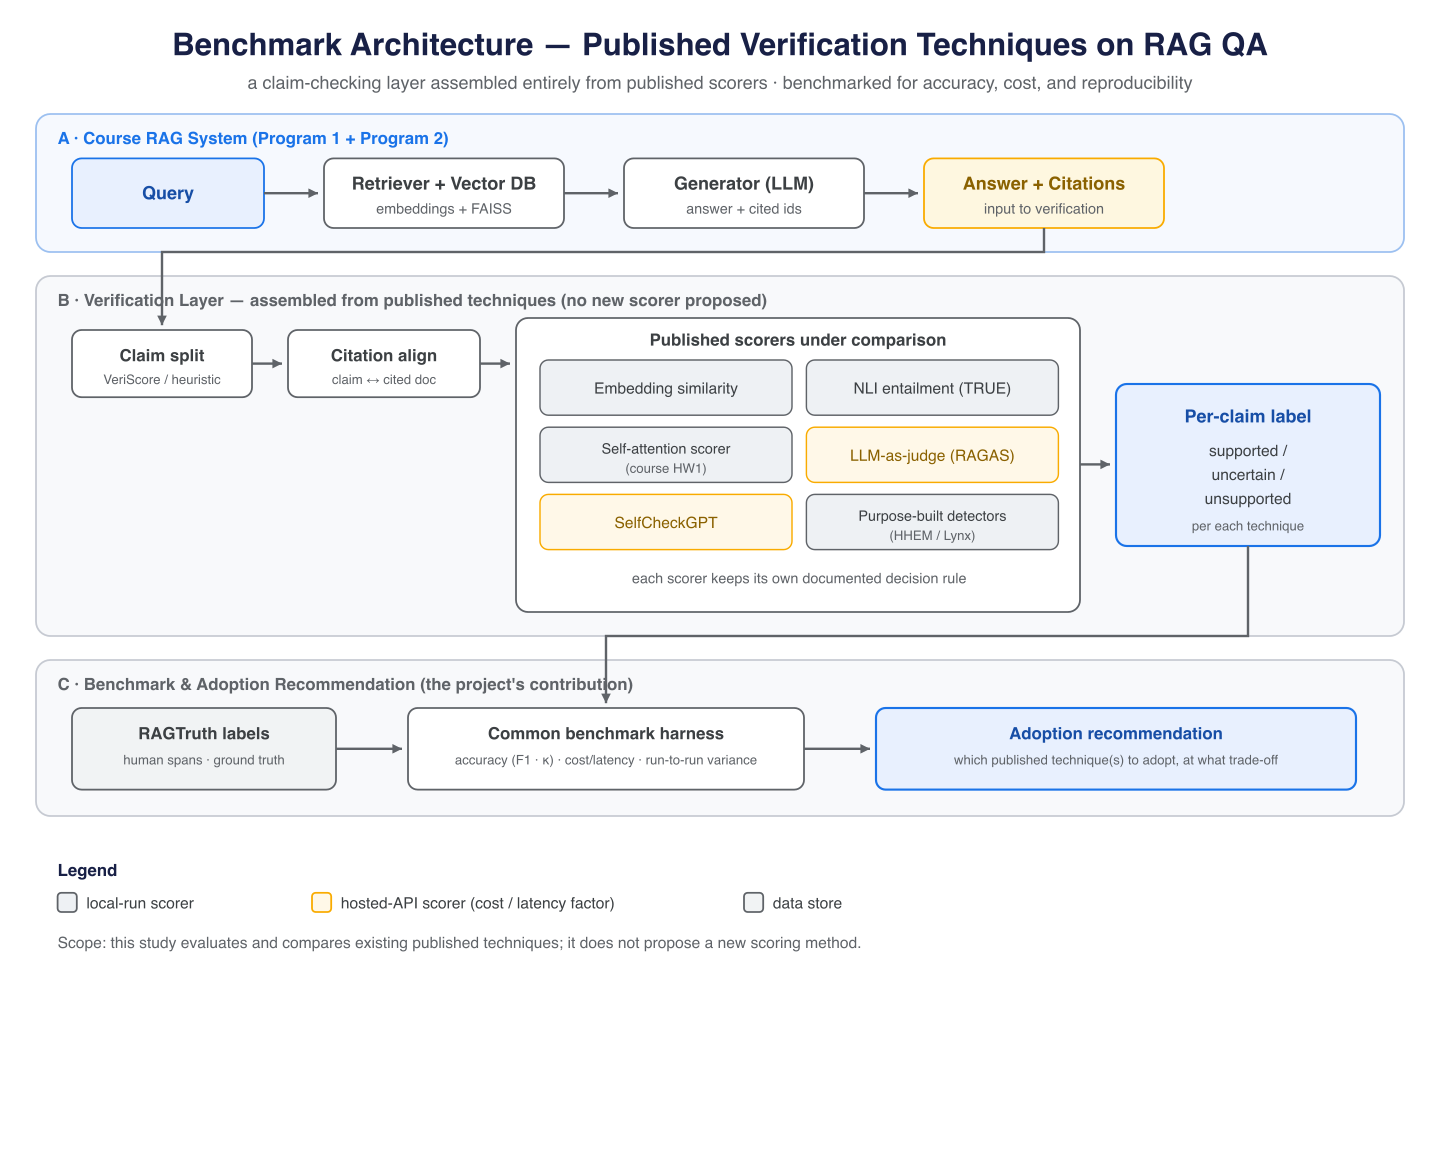
\includegraphics[width=\textwidth]{figures/bench-arch.png}
\caption{Benchmark architecture. A claim-checking layer (zone~B) assembled entirely from
published scorers is run on the course RAG system (zone~A); every technique keeps its own
documented decision rule and is scored by a common benchmark harness against RAGTruth human
labels (zone~C). The project's contribution is the comparison and the adoption
recommendation, not a new scoring method.}
\label{fig:layer}
\end{figure}


\section{Experimental Results}
\label{section:exp}
\subsection{Evaluation of Baseline Methods}
\label{section:exp:baseline}

This is a proposal; below is the planned experimental protocol and the baseline numbers
we will reproduce first.

\textbf{Planned protocol.}
\begin{enumerate}
  \item \textbf{Reproduce the floor.} Run the presence-only citation check---the one built
  into the course's Program~2, which (per its authors' note) verifies only that a citation
  id exists \citep{gao2023alce}---on RAGTruth~\citep{niu2024ragtruth} and report how many
  human-annotated unsupported spans it misses (expected: most). This quantifies the gap the
  published verification techniques must close on the provided system.
  \item \textbf{Reproduce the LLM-judge standard.} Run RAGAS faithfulness~\citep{es2024ragas}
  on the same claims and record (a) detection F1 vs.\ human labels, (b) run-to-run verdict
  variance under identical inputs, and (c) API cost/latency per 1k claims.
  \item \textbf{Evaluate the non-LLM-judge scorers.} Apply the NLI and
  embedding-similarity scorers (and the course HW1 self-attention scorer) with their
  documented decision rules; report detection P/R/F1, $\kappa$ vs.\ humans, determinism,
  and cost on the test split.
  \item \textbf{Ablations.} encoder choice; claim-segmentation granularity; a combined
  embedding$+$NLI decision.
\end{enumerate}

\textbf{Reporting template (to be filled with measured numbers).}
\begin{center}
\begin{tabular}{lcccc}
\toprule
Method & Detection F1 & $\kappa$ vs.\ human & Determinism (var) & Cost / 1k claims \\
\midrule
Presence-only \citep{gao2023alce}      & TBD & TBD & $0$ & $\approx 0$ \\
LLM-judge (RAGAS) \citep{es2024ragas}  & TBD & TBD & $>0$ (measured) & API \\
NLI-based \citep{honovich2022true}     & TBD & TBD & $0$ & GPU \\
Embedding-similarity (bge-m3)          & TBD & TBD & $0$ & no judge calls \\
Self-attention scorer (course HW1)     & TBD & TBD & $0$ & no judge calls \\
\bottomrule
\end{tabular}
\end{center}

\textbf{Success criterion.} The study succeeds if it produces a clear, evidence-based
recommendation: which published verification technique(s) give the best
accuracy/cost/reproducibility trade-off as a RAG verification layer, and where a
lightweight non-LLM-judge scorer suffices versus where a heavier method is needed---an
honest comparative result either way.


\section{Expected Contributions of Each Team Member}

We work in a shared repository with a common evaluation harness so members can work in
parallel and integrate through fixed data and metric contracts. (Allocation is tentative
and will be rebalanced as we proceed.)

\begin{itemize}
    \item \textbf{Mei-Chen (Emma) Wu (414551035):} verification-layer integration ---
    a character-level language-ID pre-filter (course HW1), claim segmentation and citation
    alignment, wiring the published scorers
    (embedding-similarity, NLI, and the course HW1 self-attention scorer) behind a common
    interface, and the metric harness (detection F1, $\kappa$, determinism, cost).
    \item \textbf{Chun-Yao Tseng (315551125):} RAG base + benchmarks --- stand up the
    course Program~1/Program~2 (vector DB $+$ cited QA), load RAGTruth/Face4RAG/FaithBench
    and the human-labeled configuration subset, and run the LLM-judge (RAGAS) and
    purpose-built detector baselines.
    \item \textbf{Bo-Yu Xu (315511057):} analysis + writing --- the
    accuracy/cost/reproducibility comparison, the adoption recommendation, figures/tables,
    and the final report.
    \item \textbf{Noa Andre (315554801):} survey + data --- the review of published
    faithfulness-verification techniques (RAGAS, FActScore, NLI, VeriScore, RAGTruth,
    FaithBench, Face4RAG), dataset curation and preprocessing of the evaluation corpora,
    and reproducibility packaging of the released splits and configs.
\end{itemize}

The two load-bearing deliverables are (1)~a fair comparison of \emph{published}
verification techniques on one RAG system and (2)~a reproducible adoption recommendation.


\newpage
{
\small
\bibliographystyle{unsrtnat}
\bibliography{reference}
}


\end{document}
